\section{Dataset and Evaluation}

The competition has three major components. 
The first are the metadata associated with the competition comprising a presence-only training, presence-absence training, and presence-absence test set. 
The metadata provides a mapping between location and the species labels available for supervised training. 
The second are the remote-sensing and raster data provided in pixel format. 
The final component is time series data containing quarterly environmental data over a 20 year period. 

The presence-only training dataset comprises 5M examples over 4M survey sites distributed across Western Europe.
The presence-absent dataset data of a similar schema, but the semantics are stricter -- species not included in the survey are known to be absent. 
This is not necessarily the case with the present-only data since they are scraped from crowd-sourced data, meaning there may be gaps in reported species. 
The datasets include an identifier for the survey site and the latitude and longitude. 
We compute a projection into EPSG 3035, which allows for Euclidean distance in units of meters. 

\begin{table}[ht]
\centering
\caption{Number of survey identifiers per dataset.}
\label{lst:counts}
\begin{tabular}{|c|c|}
\hline
dataset   & count   \\ \hline
po        & 5079797 \\ \hline
pa\_train & 1483637 \\ \hline
pa\_test  & 4716    \\ \hline
\end{tabular}
\end{table}

\begin{lstlisting}[caption={Schema of the metadata.}, captionpos=b,label={lst:schema},frame=single]
  |-- dataset: string (nullable = true)
  |-- surveyId: integer (nullable = true)
  |-- lat_proj: double (nullable = true)
  |-- lon_proj: double (nullable = true)
  |-- lat: double (nullable = true)
  |-- lon: double (nullable = true)
  |-- year: integer (nullable = true)
  |-- geoUncertaintyInM: double (nullable = true)
  |-- speciesId: double (nullable = true) 
\end{lstlisting}

The raster and satellite imagery accounts for the majority of the available data. 
We are provided GeoTIFF files for various measures such as elevation, roads, population, and soil. 
The GeoTIFF files are bounded by a GeoJSON polygon that covers Western Europe. 
RGB-NIR satellite imagery is provided directly as tiles associated with each survey site.

\begin{figure}
\begin{lstlisting}[frame=single]
  {
    "type": "Polygon",
    "coordinates": [
        [
            [-32.26344, 26.63842],
            [-32.26344, 72.18392],
            [35.58677, 72.18392],
            [35.58677, 26.63842],
            [-32.26344, 26.63842],
        ]
    ],
}
\end{lstlisting}
\caption{GeoJSON polygon for region specified by GeoLifeCLEF 2024.}
\label{lst:polygon}
\end{figure}

\subsection{Processing Raster Data}

We process GeoTIFF files for use within a supervised learning process. 
There is significant in-memory overhead with tiling the data since we need to store the 128x128 byte array for each survey site. 
We fork the official \texttt{plantnet/GeoLifeCLEF} data loaders to pre-compute tiles for each of the provided GeoTIFF under 1GB. 
Certain rasters do not fit into memory (e.g., elevation raster at 11GB); therefore, we omit them from our experiments. 
We only compute the tiles associated with the survey identifiers in our metadata, which helps limit the size of the resulting dataset. 
In addition to generating tiled images, we compute the 2D-DCT on the resulting tile images and keep low-frequency coefficients as features in downstream modeling. 


\begin{figure}[h!]
    \centering
    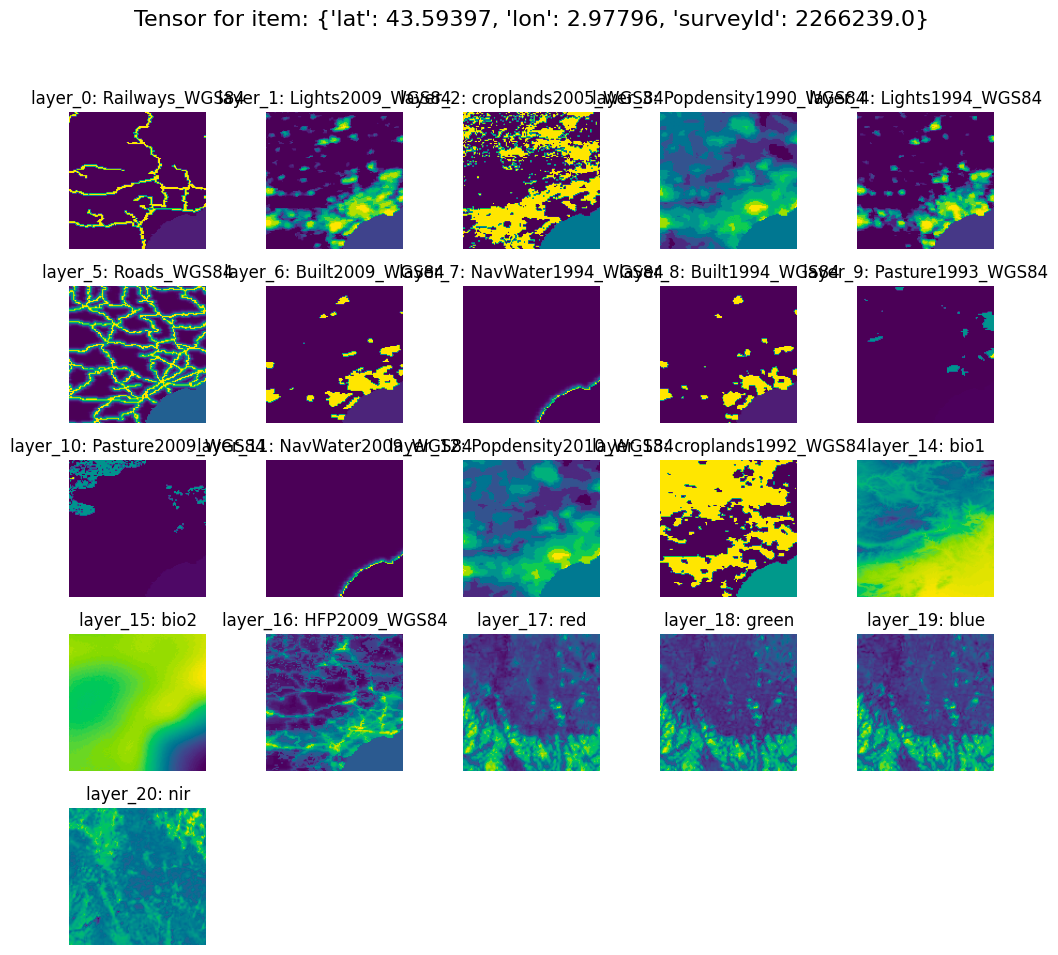
\includegraphics[width=0.9\textwidth]{figures/tiled-raster.png}
    \caption{
        Example of a tiled raster image. 
        The image is a 128x128 tile of the RGB-NIR satellite imagery. 
        The image is associated with a survey site and is used as input to the model. 
    }
    \label{fig:tiled-raster}
\end{figure}

We implement a wrapper around the ND-DCT that we can use in Spark. 
While we can access a native 1D-DCT implementation for feature pre-processing, we lose significant spatial information if we flatten the image and run a low-pass filter as seen in figure \ref{fig:dct-lowpass}.

% three images side by side
\begin{figure}
  \centering
  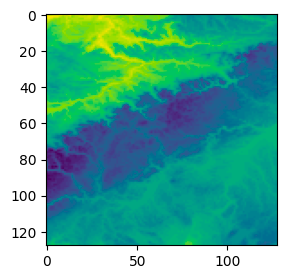
\includegraphics[width=0.3\textwidth]{figures/dct-original.png}
  \hfill
  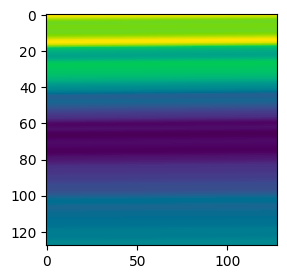
\includegraphics[width=0.3\textwidth]{figures/dct-1d-lowpass.png}
  \hfill
  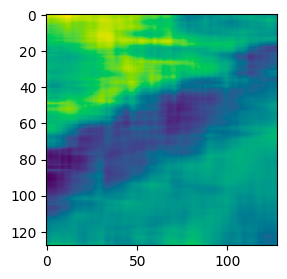
\includegraphics[width=0.3\textwidth]{figures/dct-2d-lowpass.png}
  \caption{
    Example of low-pass filtering using the DCT.
    (a) Original bio1 raster image.
    (b) Low-pass filter using the first 50 coefficients of the 1D-DCT, reshaping on the first axis (row-major order).
    (c) Low-pass filter using the 2D-DCT using the top-left 8x8 coefficients.
  }
  \label{fig:dct-lowpass}
\end{figure}

\subsection{Processing Time-Series Data}

In addition to the raster data, we process time series data so they fit within our modeling framework.
We have access to quarterly time-series data for each survey site over 20 years.
Some sites have missing data, which we pad with zeros.
We compute the 1D DCT on the time series data and keep the low-frequency coefficients as features in downstream modeling.
We keep the first 64 coefficients in the transformed space, which we choose to parallel with the 8x8 2D-DCT coefficients extracted from the raster data.
As shown in Figure \ref{fig:dct-timeseries}, the original time-series data and its DCT are displayed side by side.


% two images side by side
\begin{figure}[h!]
  \centering
  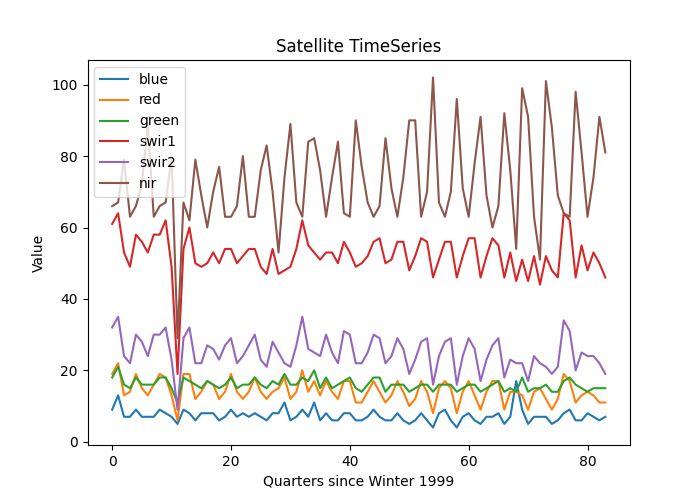
\includegraphics[width=0.495\textwidth]{figures/6-bands.png}
  \hfill
  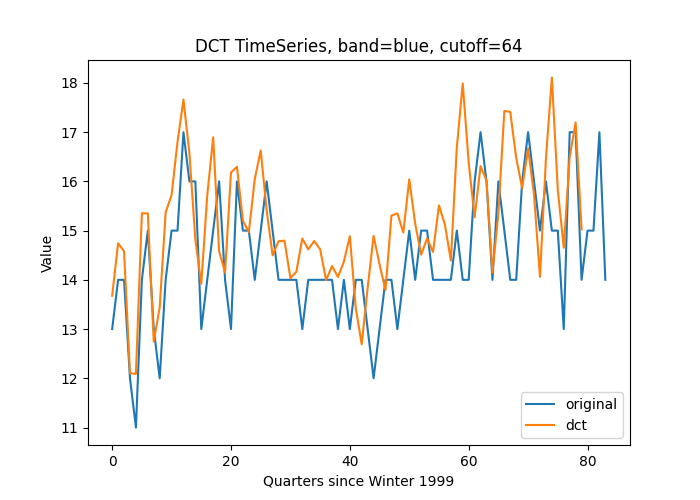
\includegraphics[width=0.495\textwidth]{figures/both.png}
  \caption{
    Example of time-series data and its DCT.
    (a) Original time-series data.
    (b) Blue band time-series approximated using DCT.
  }
  \label{fig:dct-timeseries}
\end{figure}
\subsection{Raster Data Augmentation}

We apply augmentations to our data to encourage model invariance to rotation and reflection.
We can implement augmenting transforms in pixel space by rotating and flipping images before sending them into a model.
Equivalent augmentations exist in frequency space.
For example, a 90-degree rotation in pixel space is equivalent to the transpose of the 2D-DCT coefficients.
We can flip the image in pixel space by alternating the signs of the 2D-DCT coefficients along a given axis.
Rotations and flips along the axis give us enough flexibility to implement useful symmetries in the data to improve generalization.

\begin{figure}
\begin{lstlisting}[language=Python,frame=single]
class DCTHorizontalFlip:
    def __init__(self, k=8):
        self.odd_factor = -torch.ones((k, k))
        for i in range(0, k, 2):
            self.odd_factor[i, :] = 1

    def forward(self, X):
        return X * self.odd_factor
\end{lstlisting}
\caption{Augmentation of 2D-DCT coefficients.}
\label{lst:augmentation}
\end{figure}